\chapter{电极动力学与电分析}\label{ch:b3:electrode-kinetics}

一滴血滴在塑料试条上，五秒钟后显示一个数字：血糖仪
数百万人每天要用好几次，它是一个电化学池，
它测量的是电流而非电压。一种酶使葡萄糖氧化，
一种溶解的铁配合物将电子传给碳
电极，流过的电流大小由该配合物扩散到电极的快慢决定，
因此取决于其浓度。本章解释为何
电子穿过界面快或慢（巴特勒–福尔默方程），
传质如何限制电流，以及循环伏安法等其他
电分析方法如何将电流转化为浓度、速率常数
与反应机理。

\begin{recall}
本科一年级分册定义了电极电势、标准电极电势、
能斯特方程、参比电极与半电池。本科二年级分册
介绍了电流–电势曲线及阳极电流、阴极电流，
工作电极与对电极、过电势、快速与慢速体系、
扩散层与极限电流；活度系数与离子
强度；标准曲线、标准加入法与检出
限。\Cref{ch:b3:rate-theories}介绍了过渡态理论。从
物理学中的菲克定律、泊松方程与电容器。
\end{recall}

\begin{omfigure}
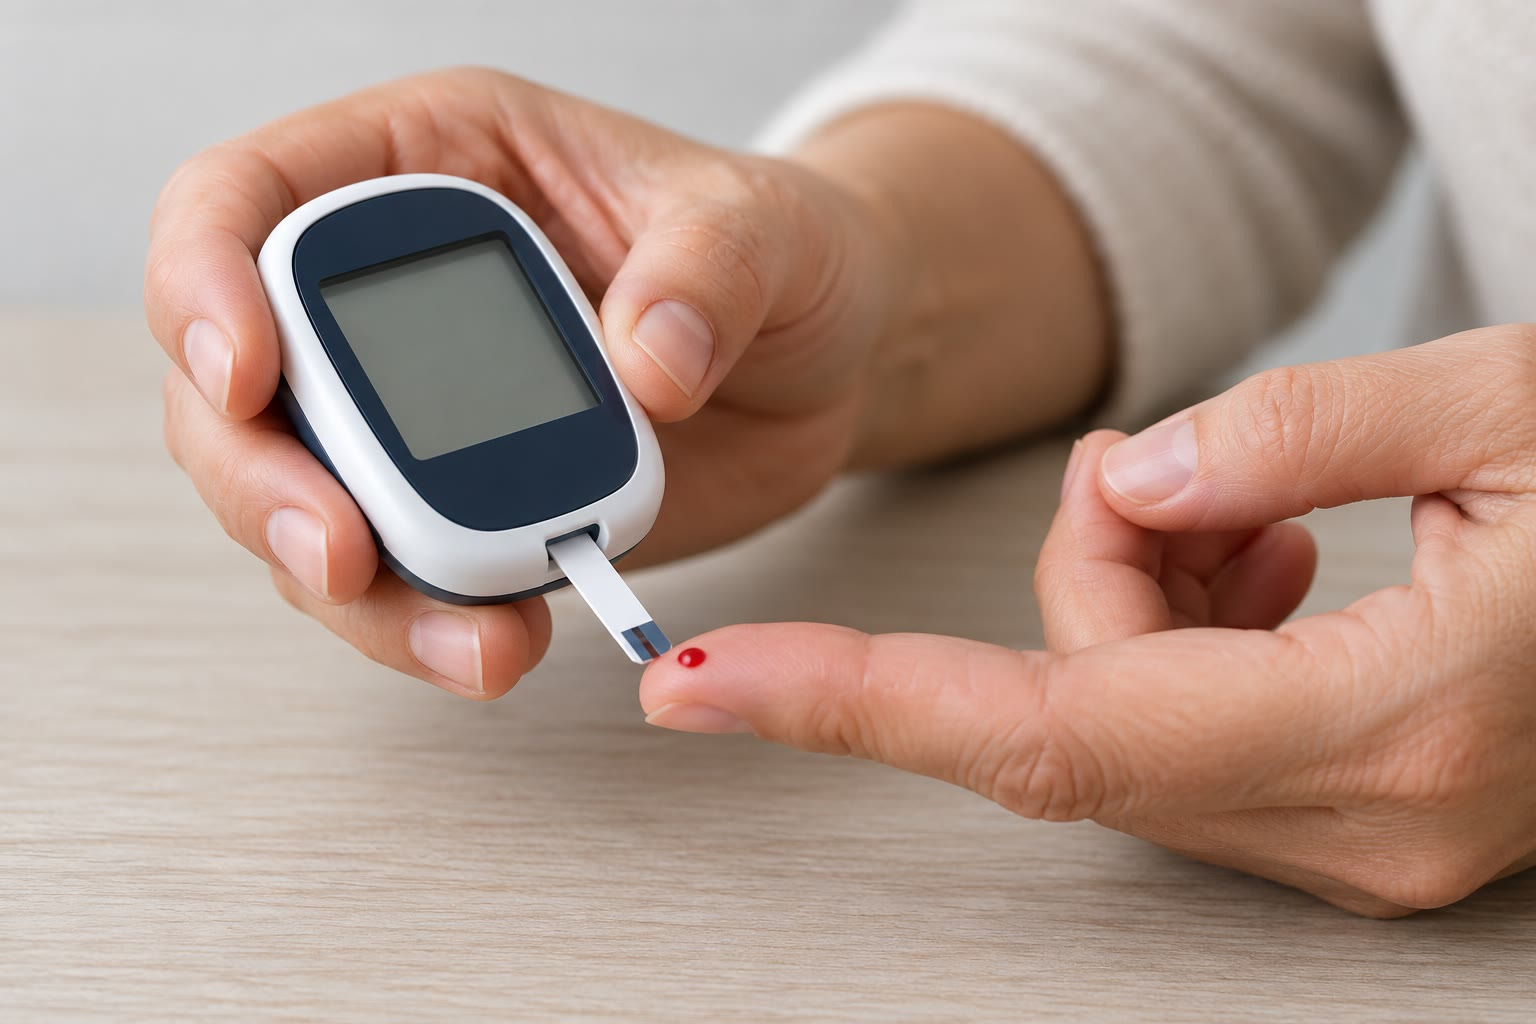
\includegraphics[width=0.6\linewidth]{images/book4/ai/b3-15-glucose-meter.jpg}

{\small 血糖仪示意：试条上带有一个微型三电极电化学池，
内含一种酶和一种氧化还原介体；仪器施加电势并读取
电流。}
\end{omfigure}

\section{电极–溶液界面}

金属插入电解质溶液后带有表面电荷，
溶液则以等量异号的电荷与之对应，该电荷由过量
同一符号的离子构成。两层电荷构成分子厚度的电容器。

\begin{definition}[双电层]\label{def:b3:electrode-kinetics:double-layer}
称\emph{双电层}\index{双电层}为电极–溶液界面上的
电荷分布：金属上的电荷与溶液中
用以补偿的离子电荷。其紧密部分，即
\emph{亥姆霍兹层}\index{亥姆霍兹层}，是与表面接触的离子与
溶剂分子所构成的层；其\emph{扩散层}\index{扩散层}
位于其外侧，热运动使过量离子分散开来，
范围约为\emph{德拜长度}\index{德拜长度} $\kappa^{-1}$ 的数量级。
\emph{双电层电容}\index{双电层电容} $C_{\mathrm{dl}}$ 是界面上
每伏电势差下单位面积所储存的电荷。
\end{definition}

\begin{proposition}[德拜长度]\label{prop:b3:electrode-kinetics:debye-length}
在离子强度为 $I$（单位 \unit{mol.m^{-3}}）、相对介电常数为
$\varepsilon_r$ 的溶液中，电极处的微小电势 $\varphi_0$ 按
$\varphi = \varphi_0\eu^{-\kappa x}$ 的形式衰减，其中
\[
  \kappa^{-1} = \sqrt{\frac{\varepsilon_r\varepsilon_0RT}{2F^2I}} .
\]
\end{proposition}

\begin{proof}
泊松方程（来自物理学）将电势与电荷密度联系起来：
$\dd^2\varphi/\dd x^2 = -\rho/\varepsilon_r\varepsilon_0$。每种离子在电势中
服从玻尔兹曼分布：$c_i = c_i^{\circ}\eu^{-z_iF\varphi/RT}$，于是 $\rho = F\sum_iz_ic_i^{\circ}\eu^{-z_iF\varphi/RT}$。当 $F\varphi \ll RT$ 时，
$\eu^{-z_iF\varphi/RT} \approx 1 - z_iF\varphi/RT$；零阶项因电中性而抵消，
且 $\rho \approx -(F^2/RT)\sum_iz_i^2c_i^{\circ}\,\varphi = -(2F^2I/RT)\varphi$。由此 $\dd^2\varphi/\dd x^2 = \kappa^2\varphi$，其
远处为零的解为 $\varphi_0\eu^{-\kappa x}$。
\end{proof}

\begin{example}[双电层的厚度]\label{ex:b3:electrode-kinetics:debye}
% ledger: eps:H2O.25C, const:eps0, const:F, const:R
在 \qty{298.15}{K} 的水中（$\varepsilon_r = 78.4$），含 \qty{0.10}{mol/L} 的 1:1 型盐（$I = \qty{100}{mol.m^{-3}}$）时，
$\kappa^{-1} = \sqrt{78.4 \times \num{8.854e-12} \times 2479/(2 \times 96\,485^2 \times 100)} = \qty{0.96}{nm}$；在 \qty{1.0}{mmol/L} 时，
厚度约为前者的十倍。支持电解质可将扩散层压缩至
几个分子直径的尺度。
\end{example}

扩散层的行为类似极板间距为 $\kappa^{-1}$ 的电容器，其
低电势下单位面积的电容为 $\varepsilon_r\varepsilon_0\kappa$（古依–查普曼
结果；其对电势的依赖关系在本阶段不加证明地承认）。与
紧密的亥姆霍兹层串联，得到实测的 $C_{\mathrm{dl}}$，数量级为数十
微法每平方厘米（斯特恩模型）。电势一旦变化，该电容器
即充电：扫描速率为每秒 $v$ 伏时，产生充电电流 $C_{\mathrm{dl}}Av$，
它不含化学信息，却会叠加到每一次伏安测量中。

\begin{omfigure}
\begin{tikzpicture}[font=\small, >=Stealth]
  \fill[black!25] (-1.0,0) rectangle (0,3.2);
  \node[rotate=90] at (-0.5,1.6) {金属};
  \foreach \y in {0.3,0.8,...,2.9}{\node[font=\scriptsize] at (-0.15,\y) {$-$};}
  \foreach \y in {0.35,0.95,1.55,2.15,2.75}{\draw[omDef, fill=omDef!20] (0.3,\y) circle (0.18); \node[font=\scriptsize] at (0.3,\y) {$+$};}
  \draw[black!50, dashed] (0.55,0) -- (0.55,3.2);
  \node[font=\scriptsize, anchor=south, align=center] at (0.45,3.25) {亥姆霍兹 \\ 面};
  \foreach \x/\y/\s in {1.1/0.6/+, 1.4/2.2/+, 1.9/1.3/+, 2.3/2.7/-, 2.6/0.5/+, 3.1/1.8/+, 3.5/0.9/-, 3.9/2.4/+, 4.4/1.4/-, 4.8/0.4/+, 5.1/2.8/-, 5.4/1.9/+}{
    \draw[black!60, fill=white] (\x,\y) circle (0.15); \node[font=\scriptsize] at (\x,\y) {$\s$};}
  \node[font=\scriptsize, anchor=south] at (3.2,3.25) {扩散层};
  \draw[->] (0,-2.1) -- (6.0,-2.1) node[anchor=north east] {$x$};
  \draw[->] (0,-2.1) -- (0,-0.3) node[anchor=east] {$|\varphi|$};
  \draw[omThm, thick] (0,-0.5) -- (0.55,-1.0) plot[domain=0.55:5.8, samples=40] (\x,{-2.1+1.1*exp(-(\x-0.55)/1.2)});
  \draw[black!40, dashed] (0.55,-2.1) -- (0.55,-0.4);
  \node[omThm, anchor=south west] at (1.3,-1.6) {$|\varphi(x)|$};
  \draw[<->, black!60] (0.55,-2.5) -- (1.75,-2.5) node[midway, below, font=\scriptsize] {$\sim\kappa^{-1}$};
\end{tikzpicture}

{\small 双电层（古依–查普曼–斯特恩模型，示意）：一
带负电的金属、位于亥姆霍兹面的紧密阳离子层，
以及扩散层，在数个德拜长度范围内阳离子多于阴离子。
下方为电势大小（负值，与金属所带电荷同号）随
距离在紧密层中线性下降，随后在扩散层中指数衰减。}
\end{omfigure}

\section{电子转移动力学}

考虑还原反应 $\mathrm{O} + n\,\mathrm{e}^- \to \mathrm{R}$，其电极电势保持为 $E$，
其在本体溶液中的平衡电势为 $E_{\mathrm{eq}}$。
过电势为 $\eta = E - E_{\mathrm{eq}}$。

\begin{definition}[交换电流密度、传递系数、标准速率常数]\label{def:b3:electrode-kinetics:exchange}
平衡时，阳极电流与阴极电流大小相等、方向相反，二者
共同的单位面积大小即为\emph{交换电流
密度}\index{交换电流密度} $j_0$。\emph{传递系数}
\index{传递系数} $\alpha$（$0 < \alpha < 1$）是
使阴极反应势垒降低的电能 $nF\eta$ 所占的份额。
\emph{标准速率常数}\index{标准速率常数} $k^\circ$ 是
阴极与阳极速率常数在形式电势 $E^{\circ\prime}$ 下的共同值。
\end{definition}

\begin{theorem}[巴特勒–福尔默方程]\label{thm:b3:electrode-kinetics:butler-volmer}
若表面浓度与本体浓度相等（无传质
限制），则在过电势 $\eta$ 下的电流密度
（阳极电流取正）为
\[
  j = j_0\bigl[\eu^{(1 - \alpha)f\eta} - \eu^{-\alpha f\eta}\bigr], \qquad f = \frac{nF}{RT}.
\]
此式称为\emph{巴特勒–福尔默方程}\index{巴特勒–福尔默方程}。
\end{theorem}

\begin{proof}
由过渡态理论，阴极与阳极速率常数分别为
$k_{\mathrm c} = A\eu^{-\Delta G_{\mathrm c}^{\ddagger}/RT}$ 与 $k_{\mathrm a} = A\eu^{-\Delta G_{\mathrm a}^{\ddagger}/RT}$。电极电势改变 $\delta E$
时，反应 $\mathrm{O} + n\,\mathrm{e}^- \to \mathrm{R}$ 的吉布斯自由能改变 $nF\,\delta E$（
金属中的电子获得 $-nF\,\delta E$ 的电能）。设一级近似下，该变化量中
比例为 $\alpha$ 的部分进入阴极势垒，其余
进入阳极势垒：$\Delta G_{\mathrm c}^{\ddagger} \to \Delta G_{\mathrm c}^{\ddagger} + \alpha nF\,\delta E$，$\Delta G_{\mathrm a}^{\ddagger} \to \Delta G_{\mathrm a}^{\ddagger} - (1 - \alpha)nF\,\delta E$。以平衡电势为起点测量 $\delta E$
此时两电流大小均为 $j_0$，
可得 $j_{\mathrm c} = j_0\eu^{-\alpha f\eta}$ 和 $j_{\mathrm a} = j_0\eu^{(1 - \alpha)f\eta}$，净电流为二者之
差。
\end{proof}

\begin{corollary}[电荷转移电阻]\label{cor:b3:electrode-kinetics:linear}
当 $|\eta| \ll RT/nF$ 时，$j = j_0f\eta$，界面表现为一个电阻
$R_{\mathrm{ct}} = RT/(nFi_0)$，其中 $i_0 = j_0A$。
\end{corollary}

\begin{proof}
将两个指数项展开到一阶：$j = j_0[(1 - \alpha)f\eta + \alpha f\eta] = j_0f\eta$；再
由此得 $\eta/i = 1/(fi_0)$。
\end{proof}

\begin{corollary}[塔费尔方程]\label{cor:b3:electrode-kinetics:tafel}
当 $\eta \ll -RT/nF$（强阴极过电势）时，阳极项
可忽略，并有
\[
  \eta = \frac{2.303\,RT}{\alpha nF}\bigl(\log j_0 - \log|j|\bigr):
\]
$\log|j|$ 与 $\eta$ 呈线性关系，每十倍电流的斜率为 $1/(\text{\qty{118}{mV}})$，在 \qty{298}{K} 下，取 $\alpha = 0.5$，$n =
1$。此式即\emph{塔费尔方程}\index{塔费尔方程}。
\end{corollary}

\begin{proof}
$|j| = j_0\eu^{-\alpha f\eta}$，故 $\ln|j| = \ln j_0 - \alpha f\eta$；换为常用对数即可。
\end{proof}

\begin{definition}[电荷转移电阻、塔费尔斜率]\label{def:b3:electrode-kinetics:charge-transfer}
电极的\emph{电荷转移电阻}\index{电荷转移电阻}
定义为 $R_{\mathrm{ct}} = (\partial\eta/\partial i)_{\eta = 0}$。\emph{塔费尔斜率}\index{塔费尔斜率}
是塔费尔区内电流每变化十倍时过电势的改变量，
即 $2.303\,RT/\alpha nF$。
\end{definition}

\begin{omfigure}
\begin{tikzpicture}
\begin{axis}[name=bv, omcv, width=0.47\linewidth, height=5.4cm, xmin=-300, xmax=300, ymin=-40, ymax=40,
  xlabel={$\eta$ / mV}, ylabel={$j/j_0$},
  legend style={font=\scriptsize, draw=none, at={(0.03,0.97)}, anchor=north west}, legend cell align=left]
\addplot[omDef, thick] table[x=eta_mV, y=a3] {figdata/out/bachelor-3-butler-volmer.dat};
\addplot[black, thick] table[x=eta_mV, y=a5] {figdata/out/bachelor-3-butler-volmer.dat};
\addplot[omThm, thick] table[x=eta_mV, y=a7] {figdata/out/bachelor-3-butler-volmer.dat};
\legend{$\alpha = 0.3$, $\alpha = 0.5$, $\alpha = 0.7$}
\draw[black!30] (axis cs:-300,0) -- (axis cs:300,0) (axis cs:0,-40) -- (axis cs:0,40);
\end{axis}
\begin{axis}[at={(bv.east)}, anchor=west, xshift=1.2cm, omcv, width=0.47\linewidth, height=5.4cm,
  xmin=-300, xmax=300, ymin=-1.5, ymax=4, xlabel={$\eta$ / mV}, ylabel={$\log|j/j_0|$},
  unbounded coords=jump]
\addplot[omDef, thick] table[x=eta_mV, y=l3] {figdata/out/bachelor-3-butler-volmer.dat};
\addplot[black, thick] table[x=eta_mV, y=l5] {figdata/out/bachelor-3-butler-volmer.dat};
\addplot[omThm, thick] table[x=eta_mV, y=l7] {figdata/out/bachelor-3-butler-volmer.dat};
\draw[black!40, dashed] (axis cs:-300,2.54) -- (axis cs:0,0);
 \draw[black!50] (axis cs:-200,1.85) -- (axis cs:-120,3.3) node[anchor=south, font=\scriptsize, inner sep=1pt] {斜率 $1/(\qty{118}{mV})$};
\end{axis}
\end{tikzpicture}

{\small 三种传递系数下的巴特勒–福尔默方程（$n = 1$，\qty{298}{K}）。左图：
平衡点附近电流与 $\eta$ 呈线性关系（即
电荷转移电阻），远离平衡时呈指数变化；$\alpha$ 使曲线不对称。
右图为塔费尔图，其直线段外推至 $\log|j/j_0| = 0$
所对应的 $\eta = 0$；虚线为 $\alpha = 0.5$ 的阴极塔费尔线。}
\end{omfigure}

\begin{method}[塔费尔分析]\label{met:b3:electrode-kinetics:tafel-analysis}
\begin{enumerate}
  \item 在搅拌溶液中记录稳态电流随 $\eta$ 的变化，电流远低于
        极限电流（或对传质进行修正）。
  \item 作 $\log|i|$ 对 $\eta$ 的图，拟合约 \qty{100}{mV} 以外的线性分支。
  \item 斜率给出 $\alpha$（阳极分支上为 $1 - \alpha$）；$\eta = 0$ 处的截距
        给出 $\log i_0$。
  \item 检验：在 $\eta = 0$ 附近，$i$ 对 $\eta$ 的斜率为 $1/R_{\mathrm{ct}} = nFi_0/RT$。
\end{enumerate}
\end{method}

本科二年级分册中的快速体系与慢速体系，正是这一
图景的两个极端：快速体系的 $j_0$ 很大，其电流–电势曲线
在平衡电势处陡然上升；慢速体系则需要很大的过电势
才有电流通过。同一反应的交换电流密度
随电极材料不同，在许多个数量级范围内变化：
析氢反应在铂上很快，而在汞上则极其缓慢。

\section{传质}

\begin{definition}[传质方式]\label{def:b3:electrode-kinetics:transport}
物种通过\emph{电迁移}\index{电迁移}到达电极，即离子在电场中的运动；
通过扩散，即沿浓度梯度方向进行；以及通过
\emph{对流}\index{对流}，即溶液整体的运动
（搅拌、旋转、流动）。\emph{支持电解质}\index{支持电解质}
是一种大量过量加入的惰性盐，承载了溶液中
几乎全部的电流，使电活性物质仅通过
扩散和对流传质。
\end{definition}

\begin{definition}[计时电流法]\label{def:b3:electrode-kinetics:chronoamperometry}
\emph{计时电流法}\index{计时电流法}在电极电势阶跃之后，
记录电流随时间的变化。
\end{definition}

\begin{theorem}[科特雷尔方程]\label{thm:b3:electrode-kinetics:cottrell}
在 $t = 0$ 时将电极电势阶跃至一个数值，使电活性物质
一到达面积为 $A$ 的平面电极便被消耗，在静止的
含支持电解质的溶液中，电流为
\[
  i = nFAc^*\sqrt{\frac{D}{\pi t}},
\]
其中 $c^*$ 为本体浓度，$D$ 为扩散系数。此式称为
\emph{科特雷尔方程}\index{科特雷尔方程}。
\end{theorem}

\begin{proof}
浓度满足菲克第二定律 $\partial c/\partial t = D\,\partial^2c/\partial x^2$，且 $c(x, 0) = c^*$，
$c(0, t) = 0$（当 $t > 0$ 时）且 $c \to c^*$（远离电极处）。函数 $c = c^*\operatorname{erf}(x/2\sqrt{Dt})$，其中
$\operatorname{erf}u = \frac{2}{\sqrt\pi}\int_0^u\eu^{-s^2}\dd s$，满足下列条件：$\operatorname{erf}0 = 0$，$\operatorname{erf}u \to 1$（当 $u \to \infty$ 时
即在 $t \to 0$ 时对每个 $x > 0$，以及远处）。令 $u = x/2\sqrt{Dt}$，
则 $\partial c/\partial t = c^*\frac{2}{\sqrt\pi}\eu^{-u^2}\partial u/\partial t = -c^*\frac{2}{\sqrt\pi}\eu^{-u^2}\frac{u}{2t}$ 与 $\partial^2c/\partial x^2 = c^*\frac{2}{\sqrt\pi}(-2u)\eu^{-u^2}\frac{1}{4Dt}$，
故菲克第二定律两端一致。电流即表面处的通量：$i =
nFAD(\partial c/\partial x)_{x = 0} = nFADc^*\frac{2}{\sqrt\pi}\frac{1}{2\sqrt{Dt}} = nFAc^*\sqrt{D/\pi t}$。（解的唯一性在
本阶段不加证明地承认。）
\end{proof}

\begin{omfigure}
\begin{tikzpicture}
\begin{axis}[name=pr, width=0.47\linewidth, height=5.2cm, xmin=0, xmax=600, ymin=0, ymax=1.08,
  axis lines=left, xlabel={$x$ / \unit{\micro m}}, ylabel={$c/c^*$},
  tick label style={font=\small}, label style={font=\small},
  legend style={font=\scriptsize, draw=none, at={(0.97,0.03)}, anchor=south east}, legend cell align=left]
\addplot[omDef, thick] table[x=x_um, y=t1] {figdata/out/bachelor-3-cottrell-profiles.dat};
\addplot[black!60, thick] table[x=x_um, y=t2] {figdata/out/bachelor-3-cottrell-profiles.dat};
\addplot[omThm, thick] table[x=x_um, y=t3] {figdata/out/bachelor-3-cottrell-profiles.dat};
\addplot[black, thick, dashed] table[x=x_um, y=t4] {figdata/out/bachelor-3-cottrell-profiles.dat};
\legend{\qty{0.1}{s}, \qty{1}{s}, \qty{4}{s}, \qty{16}{s}}
\end{axis}
\begin{axis}[at={(pr.east)}, anchor=west, xshift=1.3cm, width=0.47\linewidth, height=5.2cm,
  xmin=0, xmax=3.3, ymin=0, ymax=40, axis lines=left, xlabel={$t^{-1/2}$ / \unit{s^{-1/2}}},
  ylabel={$i$ / \unit{\micro A}}, tick label style={font=\small}, label style={font=\small}]
\addplot[omDef, very thick] table[x=tm12, y=i_uA] {figdata/out/bachelor-3-cottrell-current.dat};
\end{axis}
\end{tikzpicture}

{\small 计时电流法（模型：$D = \qty{1.0e-5}{cm^2.s^{-1}}$，$c^* = \qty{1.0}{mM}$，
圆盘电极直径为 \qty{3}{mm}）。左图：耗尽层按 $\sqrt{Dt}$ 增长，\qty{0.1}{s} 后约为 \qty{30}{\micro m}，
而 \qty{16}{s} 后约为 \qty{350}{\micro m}。右图：科特雷尔电流正比于
$t^{-1/2}$；其斜率给出 $D$。}
\end{omfigure}

搅拌溶液或旋转圆盘电极可使扩散层保持
恒定厚度 $\delta$，此时电流达到稳定极限值 $nFADc^*/\delta$
（本科二年级分册中的结果）。对旋转圆盘电极，$\delta$ 随转速的
平方根成反比减小（列维奇，在本阶段不加证明地承认），这使极限电流
正比于 $\sqrt\omega$。

\section{循环伏安法}

\begin{definition}[循环伏安法]\label{def:b3:electrode-kinetics:cv}
\emph{循环伏安法}\index{循环伏安法}令静止工作电极的电势在两个极限值之间随时间线性扫描，
往返一次，
在静止溶液中以扫描速率 $v$ 进行，并记录电流。
以电流对电势作图，所得图线称为\emph{伏安图}\index{伏安图}；每个波都有一个
\emph{峰电流}\index{峰电流} $i_{\mathrm p}$，位于其\emph{峰电势}\index{峰电势}
$E_{\mathrm p}$ 处。
\end{definition}

峰的出现源于两种相互竞争的效应：当电势越过 $E^{\circ\prime}$ 时，
反应物的表面浓度下降（对快速体系适用能斯特方程），
电流随之增大；但耗尽层随时间增厚，
通量下降。回扫时，仍靠近电极的产物被
重新转化回去。

\begin{definition}[可逆性]\label{def:b3:electrode-kinetics:reversibility}
用无量纲速率参数 $\Lambda = k^\circ/\sqrt{DnFv/RT}$，将
电子转移速率与扫描所施加的扩散速率相比较，一个电对
为\emph{电化学可逆}\index{电化学可逆}，
当 $\Lambda > 15$ 时（其表面浓度在任何时刻都服从能斯特方程），
为\emph{准可逆}\index{准可逆}，即 $15 >
\Lambda > 10^{-2(1 + \alpha)}$，而
低于此值者为\emph{电化学不可逆}\index{电化学不可逆}。
\end{definition}

\begin{remark}
本科二年级分册中的快速体系与慢速体系对应于此分类，
但有一点不同：此处的可逆性取决于扫描
速率。同一电对可以在 \qty{10}{mV/s} 下为可逆的，而在
\qty{10}{V/s} 下为准可逆的，因为扫描越快，留给电子转移的时间越少。
\end{remark}

\begin{proposition}[兰德尔斯–塞夫契克方程]\label{prop:b3:electrode-kinetics:randles-sevcik}
在 \qty{298}{K} 下，对平面电极上的可逆波，
\[
  i_{\mathrm p} = 0.4463\,nFAc^*\sqrt{\frac{nFvD}{RT}},
\]
由此可得 $i_{\mathrm p} \propto \sqrt v$。此式称为\emph{兰德尔斯–塞夫契克方程}\index{兰德尔斯–塞夫契克方程}。
\end{proposition}

\begin{proof}[部分证明]
在变量 $\xi = x\sqrt{nFv/(RTD)}$ 与 $\theta = nFvt/RT$（电位扫描以
$RT/nF$ 为单位），表面处带能斯特条件的菲克定律
除起始电位外不含其他参数：无量纲通量是一个
普适函数 $\chi(\theta)$。回到物理量纲，$i = nFAc^*\sqrt{nFvD/RT}\,\chi(\theta)$：每一电流（包括峰电流）
都与 $\sqrt v$ 成正比。0.4463 为
$\chi$ 的极大值，由数值求解得到（承认此结果；图中的模拟
可在 0.1\,\% 以内复现它）。
\end{proof}

\begin{proposition}[峰间距]\label{prop:b3:electrode-kinetics:delta-ep}
对可逆波，阴极峰与阳极峰各约偏离 \qty{28.5}{mV}$/n$，
分别位于 $E^{\circ\prime}$ 两侧（在 \qty{298}{K} 下，扫描换向电位远超过波的范围时）：
$\Delta E_{\mathrm p} \approx 57/n$ mV，与扫描速率无关；当两物种扩散系数相等时，$E_{1/2} = (E_{\mathrm{pc}} + E_{\mathrm{pa}})/2 =
E^{\circ\prime}$。
\end{proposition}

\begin{proof}[部分证明]
在前一证明的无量纲形式中，峰出现在
$\theta$ 的固定值处，即相对于 $E^{\circ\prime}$ 的固定电位处，与 $v$ 无关；
O 与 R 之间能斯特条件的对称性使阳极峰
对称分布。数值结果为承认结论；模拟给出
$\pm\qty{28.5}{mV}$，$\Delta E_{\mathrm p} = \qty{57.7}{mV}$。
\end{proof}

\begin{omfigure}
\begin{tikzpicture}
\begin{axis}[name=cv, omcv, width=0.62\linewidth, height=6.4cm, xmin=-320, xmax=320, ymin=-30, ymax=22,
  xlabel={$E - E^{\circ\prime}$ / mV}, ylabel={$i$ / \unit{\micro A}},
  legend style={font=\scriptsize, draw=none, fill=white, fill opacity=0.85, text opacity=1,
  at={(0.01,0.99)}, anchor=north west}, legend cell align=left]
\addplot[black!40, thin] table[x=E_mV, y=i_uA] {figdata/out/bachelor-3-cyclic-voltammetry-v25.dat};
\addplot[omDef!60, thin] table[x=E_mV, y=i_uA] {figdata/out/bachelor-3-cyclic-voltammetry-v50.dat};
\addplot[omDef, thick] table[x=E_mV, y=i_uA] {figdata/out/bachelor-3-cyclic-voltammetry-v100.dat};
\addplot[black, thick] table[x=E_mV, y=i_uA] {figdata/out/bachelor-3-cyclic-voltammetry-v200.dat};
\addplot[omThm, thick, dashed] table[x=E_mV, y=i_uA] {figdata/out/bachelor-3-cyclic-voltammetry-quasi.dat};
\legend{\qty{25}{mV/s}, \qty{50}{mV/s}, \qty{100}{mV/s}, \qty{200}{mV/s}, {准可逆，\qty{100}{mV/s}}}
\end{axis}
\begin{axis}[at={(cv.east)}, anchor=west, xshift=1.3cm, width=0.32\linewidth, height=5.0cm,
  xmin=0, xmax=0.5, ymin=0, ymax=30, axis lines=left, xlabel={$\sqrt v$ / \unit{(V/s)^{1/2}}},
  ylabel={$|i_{\mathrm{pc}}|$ / \unit{\micro A}}, tick label style={font=\small}, label style={font=\small}]
\addplot[only marks, mark=*, omDef] table[x=sqrtv, y=ip_uA] {figdata/out/bachelor-3-cyclic-voltammetry-ip.dat};
\addplot[black, domain=0:0.5] {60.06*x};
\end{axis}
\end{tikzpicture}

{\small 对还原过程用有限差分法模拟的循环伏安图
（模型：\qty{1.0}{mM}，$D = \qty{1.0e-5}{cm^2.s^{-1}}$，\qty{3}{mm} 圆盘，$n = 1$；阳极电流
取正值）。四种扫描速率下的可逆波：峰间距保持为 \qty{57.7}{mV}，
以 $E^{\circ\prime}$ 为中心，峰电流随 $\sqrt v$ 增大（右图，直线为
兰德尔斯–塞夫契克方程）。虚线：准可逆电对（$k^\circ = \qty{2e-3}{cm.s^{-1}}$），
扫描速率为 \qty{100}{mV/s}，峰间距为 \qty{162}{mV}，且峰值更低。}
\end{omfigure}

\begin{method}[诊断伏安图]\label{met:b3:electrode-kinetics:cv-diagnosis}
\begin{enumerate}
  \item 可逆：每一扫描速率下 $\Delta E_{\mathrm p} \approx 57/n$ mV，$|i_{\mathrm{pa}}/i_{\mathrm{pc}}| = 1$，$i_{\mathrm p} \propto \sqrt v$；
        由 $E_{1/2}$ 得 $E^{\circ\prime}$。
  \item 准可逆：$\Delta E_{\mathrm p}$ 随扫描速率增大；其数值给出 $k^\circ$。
  \item 不可逆：无回扫峰；扫描速率每增大十倍，峰电势移动
        $30/\alpha n$ mV。
  \item 后随化学步骤（EC 机理）：回扫峰小于正向峰，
        慢速扫描时如此，快速扫描时回扫峰恢复，
        因为快速扫描快于化学反应。
  \item 吸附物种：$i_{\mathrm p} \propto v$，而非 $\sqrt v$。
\end{enumerate}
\end{method}

非水溶剂中的电势（参比电极会漂移）需以
实验结束时加入的内标为基准，即
二茂铁正离子/二茂铁电对，它在大多数有机溶剂中快速且性质良好。

\begin{method}[搭建三电极测量]\label{met:b3:electrode-kinetics:three-electrode}
\begin{enumerate}
  \item 工作电极（玻碳、铂、金）新鲜抛光；
        对电极（铂丝）面积较大；参比电极
        （Ag/AgCl，或带内标的银丝）置于靠近工作
        电极处。
  \item 待测物溶液（约 1 mM），含 \qty{0.1}{mol/L} 支持
        电解质，用氩气除气（溶解氧在
        中等负电势下会被还原，并引入其自身的波）。
  \item 恒电势仪保持工作电极与参比电极之间的电势，
        并使电流在工作电极与对电极之间通过；
        参比电极中无电流通过。
\end{enumerate}
\end{method}

\begin{omfigure}
\begin{tikzpicture}[font=\small, >=Stealth]
  \begin{scope}[scale=1.5]
    \pic[transform shape] at (0,0) {beaker={0.7}{omWater!60}};
    \pic[transform shape] at (-0.45,0.35) {electrode={black!70}};
    \pic[transform shape] at (0,0.35) {electrode={black!20}};
    \pic[transform shape] at (0.45,0.35) {probe};
  \end{scope}
  \draw[thick] (-1.6,6.0) rectangle (1.6,7.2);
  \node at (0,6.6) {恒电势仪};
  \draw[thick, omDef] (-0.675,4.35) |- (-1.0,5.2) -- (-1.0,6.0);
  \draw[thick, black!60] (0,4.35) -- (0,6.0);
  \draw[thick, omThm] (0.675,5.18) |- (1.0,5.5) -- (1.0,6.0);
  \node[omDef, anchor=east, align=right, font=\scriptsize] at (-1.1,5.2) {工作};
  \node[black!70, rotate=90, anchor=north, font=\scriptsize, inner sep=1pt] at (0.06,5.35) {对电极};
  \node[omThm, anchor=west, align=left, font=\scriptsize] at (1.1,5.2) {参比};
\end{tikzpicture}

{\small 三电极电解池。恒电势仪控制工作电极
相对于参比电极的电势，参比电极无电流通过，
并驱动电流流经对电极。}
\end{omfigure}

\section{电分析方法}

\begin{definition}[安培法，生物传感器]\label{def:b3:electrode-kinetics:amperometry}
\emph{安培法}\index{安培法}在固定电势下测量电流，
电流与发生反应的物质浓度成正比。一个
\emph{生物传感器}\index{生物传感器}将生物识别元件（如
酶、抗体）与换能器相连，此处换能器为电极。
\end{definition}

在葡萄糖试纸中，葡萄糖氧化酶将葡萄糖氧化为葡萄糖酸内酯，并
由介质六氰合铁(III)酸根使其再生，后者被还原；在
电极上，电势保持在使六氰合铁(II)酸根被氧化的数值，
电流即测量所生成的介质量，每个葡萄糖生成两个：
\[
  \ce{C6H12O6 + 2 [Fe(CN)6]^3- -> C6H10O6 + 2 [Fe(CN)6]^4- + 2 H+} .
\]

\begin{definition}[阳极溶出伏安法]\label{def:b3:electrode-kinetics:stripping}
\emph{阳极溶出伏安法}\index{阳极溶出伏安法}
在固定电势下将金属离子还原沉积到电极上，
经固定时间实现金属的预富集；然后正向扫描电势，测量
金属再氧化的电流峰，其大小与
溶液中金属的浓度成正比。
\end{definition}

预富集使该方法足够灵敏，可用于饮用水中痕量铅或
镉的测定，浓度可达微克每升。由于
灵敏度取决于基体，因此须在样品本身中
采用标准加入法进行校准。

\begin{method}[结合溶出的标准加入法]\label{met:b3:electrode-kinetics:standard-addition}
\begin{enumerate}
  \item 记录样品的溶出峰，然后加入三次或更多次标准溶液，
        每次加入都使浓度增加已知量
        （加入体积很小，使稀释可忽略或予以校正）。
  \item 以峰高对加入浓度作拟合，得到一条直线。
  \item 该直线在浓度轴上的截距为样品浓度的负值；
        将直线的标准误差传递至结果。
\end{enumerate}
\end{method}

\begin{omfigure}
\begin{tikzpicture}
\begin{axis}[name=sp, omcv, width=0.47\linewidth, height=5.2cm, xmin=-600, xmax=-300, ymin=0, ymax=2.4,
  xlabel={$E$ / mV}, ylabel={$i$ / \unit{\micro A}}]
\addplot[black, thick] table[x=E_mV, y=s0] {figdata/out/bachelor-3-standard-addition-peaks.dat};
\addplot[omDef!50, thick] table[x=E_mV, y=s1] {figdata/out/bachelor-3-standard-addition-peaks.dat};
\addplot[omDef!80, thick] table[x=E_mV, y=s2] {figdata/out/bachelor-3-standard-addition-peaks.dat};
\addplot[omDef, thick] table[x=E_mV, y=s3] {figdata/out/bachelor-3-standard-addition-peaks.dat};
\end{axis}
\begin{axis}[at={(sp.east)}, anchor=west, xshift=1.3cm, width=0.47\linewidth, height=5.2cm,
  xmin=-6, xmax=16, ymin=0, ymax=2.3, axis x line=middle, axis y line=left,
  xlabel={加入的 Pb / \unit{\micro g.L^{-1}}}, ylabel={峰高 / \unit{\micro A}},
  tick label style={font=\small}, label style={font=\small},
  xlabel style={at={(0.5,-0.18)}, anchor=north}]
\addplot[black, thin] table[x=added, y=h] {figdata/out/bachelor-3-standard-addition-line.dat};
\addplot[only marks, mark=*, omDef] table[x=added, y=h] {figdata/out/bachelor-3-standard-addition-points.dat};
\node[font=\scriptsize, anchor=south] at (axis cs:-4.26,0.05) {$-c_0$};
\end{axis}
\end{tikzpicture}

{\small 铅的阳极溶出，三次标准加入（数据取自
\cref{exo:b3:electrode-kinetics:9}）。左图：溶出峰随每次加入而增大。
右图：峰高对加入浓度的最小二乘直线
与坐标轴交于样品浓度的负值处。}
\end{omfigure}

\begin{definition}[离子选择性电极，选择性系数]\label{def:b3:electrode-kinetics:ise}
\emph{离子选择电极}\index{离子选择电极}是一种电极，
其电势通过一种优先交换某一离子的膜，
取决于该离子的活度。其\emph{选择性
系数}\index{选择性系数} $K_{ij}$ 表示其对
干扰离子 $j$ 相对于主离子 $i$ 的响应。
\end{definition}

\begin{proposition}[尼科尔斯基方程]\label{prop:b3:electrode-kinetics:nikolsky}
设主离子 $i$ 的电荷为 $z_i$，干扰离子 $j$ 的电荷为 $z_j$，
\[
  E = \text{常数} + \frac{RT}{z_iF}\ln\bigl(a_i + K_{ij}a_j^{z_i/z_j}\bigr) .
\]
此即\emph{尼科尔斯基方程}\index{尼科尔斯基方程}。
\end{proposition}

\begin{proof}[部分证明]
对只透过 $i$ 的膜，跨膜的电化学势相等，
得到能斯特型电势 $\frac{RT}{z_iF}\ln a_i$ 加一个常数。
若 $j$ 能通过离子交换取代膜中的 $i$，其交换常数即定义 $K_{ij}$，
则膜表面 $i$ 的活度升高了
$K_{ij}a_j^{z_i/z_j}$（指数保证交换中电荷守恒）。详细
推导在本阶段不加证明地承认。
\end{proof}

玻璃 pH 电极是最早的离子选择电极；其钠
误差在高 pH 和高钠浓度下出现，即尼科尔斯基项。

\begin{definition}[库仑法]\label{def:b3:electrode-kinetics:coulometry}
\emph{库仑法}\index{库仑法}由物质完全电解时通过的总电荷
确定物质的量：$Q = nFn_{\text{物质}}$（法拉第
电磁感应定律），无需校准。
\end{definition}

\begin{proposition}[由标准曲线读取浓度的不确定度]\label{prop:b3:electrode-kinetics:inverse-prediction}
设标准曲线 $y = a + bx$ 由 $n$ 个标准样品拟合（残差
标准差 $s$，均值 $\bar y$，$S_{xx} = \sum(x_i - \bar x)^2$），
对 $m$ 次平行测量平均响应为 $y_0$ 的样品，其浓度为 $x_0 = (y_0 - a)/b$，其
标准不确定度为
\[
  u(x_0) = \frac{s}{b}\sqrt{\frac1m + \frac1n + \frac{(y_0 - \bar y)^2}{b^2S_{xx}}} .
\]
\end{proposition}

\begin{proof}
记 $x_0 = \bar x + (y_0 - \bar y)/b$。一阶近似下其方差为 $(\operatorname{var}y_0 +
\operatorname{var}\bar y)/b^2 + (y_0 - \bar y)^2\operatorname{var}b/b^4$，三项彼此不相关（$\bar y$ 与 $b$
不相关，由\cref{prop:b3:rate-theories:slope-uncertainty}可知）。代入 $\operatorname{var}y_0 =
s^2/m$，$\operatorname{var}\bar y = s^2/n$，$\operatorname{var}b = s^2/S_{xx}$，即得结论。
\end{proof}

不确定度在标准曲线范围中部最小，
越靠近两端越大；对样品的平行测量只减小第一项。

\begin{inthelab}[制备玻璃碳电极]
电极在毡垫上用氧化铝浆料
以八字形运动抛光，冲洗，在水中短时超声，再次冲洗。
已知电对（六氰合铁酸根、二茂铁）的伏安图可用来检验
峰间距是否接近可逆体系的理论值，间距较大则说明
电极表面受污染或存在未补偿电阻。溶液用氩气除气
十分钟，扫描期间始终置于氩气保护之下。
\end{inthelab}

\begin{safety}{\ghs[0.62cm]{GHS03}\ghs[0.62cm]{GHS05}\ghs[0.62cm]{GHS07}\ghs[0.62cm]{GHS08}\ghs[0.62cm]{GHS09}}
% ledger: ghs4:PbNO32, ghs4:K3FeCN6
硝酸铅（用于铅标准溶液）：具有氧化性，可能损害生育能力并
危害未出生的胎儿，疑似致癌，对水生生物毒性很大；标准溶液
须购买现成配制的，操作时戴手套，所有含铅废物须
收集。六氰合铁(III)酸钾：有害，疑似损害
生育力；切勿强酸化或加热（否则可能释放
氰化氢）。汞电极曾广泛用于溶出分析，现已
被铋膜电极和碳电极所取代。
\end{safety}

\begin{history}[海洛夫斯基的极谱仪，1922 年]
雅罗斯拉夫·海洛夫斯基于 1922 年测量了流经汞电极的电流，
汞滴从细毛细管中滴下，每隔数秒更新一次表面，
对所加电势作图。每种可还原物质给出一个波，
波的位置可用来鉴别该物质，波高则表示其浓度；
1924 年，他与志方益三合作制成了极谱仪，该仪器能
自动将曲线记录在感光纸上。极谱法是最早
投入常规应用的仪器化学分析方法，并为海洛夫斯基赢得 1959 年诺贝尔
化学奖。
\end{history}

\section{练习}

\begin{exercise}[$\star$]\label{exo:b3:electrode-kinetics:1}
某还原过程的塔费尔图（$n = 1$，\qty{298}{K}）的阴极斜率为 $-\qty{118}{mV}$
每十倍电流，外推至 $\eta = 0$ 时 $|j| = \qty{2.0e-6}{A.cm^{-2}}$（题中数据）。
求 $\alpha$ 与 $j_0$。
\end{exercise}

\begin{exercise}[$\star$]\label{exo:b3:electrode-kinetics:2}
某电极面积为 \qty{0.20}{cm^2}，对单电子电对的 $j_0 = \qty{1.0e-3}{A.cm^{-2}}$。
求其在 \qty{298}{K} 下的电荷转移电阻。
\end{exercise}

\begin{exercise}[$\star$]\label{exo:b3:electrode-kinetics:3}
% ledger: eps:H2O.25C
求 \qty{298.15}{K} 下水中，浓度分别为 \qty{1.0}{mmol/L} 与 \qty{0.10}{mol/L}
的 \ce{MgSO4} 溶液的德拜长度。
\end{exercise}

\begin{exercise}[$\star$]\label{exo:b3:electrode-kinetics:4}
在 \qty{0.0707}{cm^2} 电极上以 \qty{100}{mV/s} 扫描得到循环伏安图，双电层电容 $C_{\mathrm{dl}} =
\qty{20}{\micro F.cm^{-2}}$：求充电电流，并与图中的
\qty{19}{\micro A} 法拉第峰相比较。在 \qty{10}{V/s} 时会怎样？
\end{exercise}

\begin{exercise}[$\star\star$]\label{exo:b3:electrode-kinetics:5}
电势阶跃后，$i\sqrt t = \qty{12.2}{\micro A.s^{1/2}}$，此为单电子还原
\qty{1.00}{mM} 溶液在 \qty{0.0707}{cm^2} 电极上的结果。求 $D$。
\end{exercise}

\begin{exercise}[$\star\star$]\label{exo:b3:electrode-kinetics:6}
用兰德尔斯–塞夫契克方程求 $n = 1$、$A = \qty{0.0707}{cm^2}$、$c^* = \qty{2.0}{mM}$ 时的峰电流，
$D = \qty{7.0e-6}{cm^2.s^{-1}}$，扫描速率分别为 \qty{50}{mV/s} 与 \qty{500}{mV/s}。
\end{exercise}

\begin{exercise}[$\star\star$]\label{exo:b3:electrode-kinetics:7}
三个电对在扫描速率 50 与 \qty{500}{mV/s} 下分别给出：(a) $\Delta E_{\mathrm p} = 58$ 与 59 mV，$|i_{\mathrm{pa}}/i_{\mathrm{pc}}| = 1.0$；
(b) $\Delta E_{\mathrm p} = 75$ 与 140 mV，$|i_{\mathrm{pa}}/i_{\mathrm{pc}}| = 1.0$；(c) 在 \qty{50}{mV/s} 下 $\Delta E_{\mathrm p}$ 无定义（无
回扫峰），在 \qty{500}{mV/s} 下有回扫峰，且 $|i_{\mathrm{pa}}/i_{\mathrm{pc}}| = 0.8$。逐一判断其可逆性。
\end{exercise}

\begin{exercise}[$\star\star$]\label{exo:b3:electrode-kinetics:8}
某钾离子选择电极的 $K_{\ce{K+},\ce{Na+}} = \num{2e-4}$。在某样品中 $a(\ce{K+}) =
\qty{4.0e-3}{}$，$a(\ce{Na+}) = 0.14$，若忽略
钠离子，则钾离子活度的相对误差是多少？
\end{exercise}

\begin{exercise}[$\star\star$]\label{exo:b3:electrode-kinetics:9}
向某水样中分别加入 0、5、10 与 \qty{15}{\micro g.L^{-1}} 的铅，
所得溶出峰电流分别为 0.468、1.003、1.571 与 \qty{2.101}{\micro A}（题中数据）。求
被测溶液中铅的浓度及其标准不确定度。
\end{exercise}

\begin{exercise}[$\star\star\star$]\label{exo:b3:electrode-kinetics:10}
一台铜库仑计通以恒定的 \qty{50.0}{mA} 电流 \qty{30.0}{min}，
并自 \ce{Cu^{2+}} 中沉积出铜。求沉积物的质量；为何库仑法无需
校准？
\end{exercise}

\begin{exercise}[$\star\star\star$]\label{exo:b3:electrode-kinetics:11}
对于 $k^\circ = \qty{1.0e-2}{cm.s^{-1}}$、$D = \qty{1.0e-5}{cm^2.s^{-1}}$ 的电对，求扫描速率为 \qty{0.1}{V/s}
时的 $\Lambda$ 与 \qty{10}{V/s} 时的值（$n = 1$，\qty{298}{K}），并判断各扫描速率下波的类型。
\end{exercise}

\begin{exercise}[$\star\star\star$]\label{exo:b3:electrode-kinetics:12}
由 $n = 7$ 个标准样品得到的标准曲线，有 $b = \qty{0.919}{\micro A.mM^{-1}}$，$s = \qty{0.077}{\micro A}$，
$\bar y = \qty{8.89}{\micro A}$，$S_{xx} = \qty{241}{mM^2}$。求由读数得到的浓度的不确定度，
分别取单次读数 $y_0 = \bar y$ 与 $y_0 = \qty{18.0}{\micro A}$，以及 $\bar y$ 处的三次读数。
\end{exercise}

\section{问题：葡萄糖试纸}

\begin{problem}[{周末问题——葡萄糖试纸：酶及其
介体、计时电流法与扩散系数、标定
直线、血样及其不确定度，以及
抗坏血酸的干扰}]
\label{pb:b3:electrode-kinetics:1}
% ledger: const:F
试纸上载有葡萄糖氧化酶、六氰合铁(III)酸钾和一支
碳工作电极，面积为 \qty{0.0300}{cm^2}。本题数据：(a) 一条试纸
充有 \qty{10.0}{mM} 六氰合铁(II)酸根，并阶跃至氧化电势，
测得电流 42.0、29.3、24.1、20.8 和 \qty{18.7}{\micro A}，对应时刻 1、2、3、4 和 \qty{5}{s}；
(b) 葡萄糖标准溶液的浓度分别为 2.0、4.0、6.0、8.0、10.0、15.0 和 \qty{20.0}{mM}，
在 \qty{5.0}{s} 时测得电流依次为 2.16、4.08、5.83、7.78、9.45、14.23 和 \qty{18.69}{\micro A}；(c) 一血样
测得 \qty{7.10}{\micro A}。

\medskip\noindent\textbf{第一部分——化学原理。}
\begin{enumerate}
  \item 写出葡萄糖（生成葡萄糖酸内酯，\ce{C6H10O6}）及介体的半反应，
        并写出配平的总反应。
  \item 每个葡萄糖分子有多少个电子到达电极？
  \item 为什么使用介体代替氧气，
        氧气是该酶的天然电子受体？
  \item 为什么电极要保持在六氰合铁(II)酸根
        被氧化、远高于其形式电势的电势下？
  \item 为什么必须在液滴加到试纸上后
        的固定时刻读数？
\end{enumerate}

\medskip\noindent\textbf{第二部分——计时电流法。}
\begin{enumerate}[resume]
  \item (a) 中的电流应遵循哪一定律？请用数据检验。
  \item 以 $i$ 对 $t^{-1/2}$ 作过原点拟合，斜率为 \qty{41.8}{\micro A.s^{1/2}}。由此推算
        六氰合铁(II)酸根的 $D$。
  \item 计算 \qty{5}{s} 后耗尽层的厚度 $\sqrt{\pi Dt}$。
        平面模型对溶液层约为
        \qty{100}{\micro m} 厚的试纸是否合理？
  \item 若浓度为 \qty{5.0}{mM} 而非 \qty{10.0}{mM}，则 \qty{5}{s} 时电流为多少？
\end{enumerate}

\medskip\noindent\textbf{第三部分——标定。}
\begin{enumerate}[resume]
  \item 由 (b) 的最小二乘直线得 $a = \qty{0.356}{\micro A}$（$s_a = 0.054$），$b =
        \qty{0.9189}{\micro A.mM^{-1}}$（$s_b = 0.0049$），$s = \qty{0.077}{\micro A}$。$a$ 代表什么？
  \item 该范围内响应是否呈线性？高
        葡萄糖浓度下，什么会限制线性？
  \item 计算血样中的葡萄糖浓度。
  \item 已知 $\bar y = \qty{8.89}{\micro A}$，$S_{xx} = \qty{241}{mM^2}$，计算其标准不确定度。
  \item 不确定度中哪一项占主导？如何减小它？
  \item 以 $3s/b$ 估算检出限。
  \item 以毫克每分升表示结果（葡萄糖的摩尔质量
        为 \qty{180.16}{g/mol}）。
\end{enumerate}

\medskip\noindent\textbf{第四部分——干扰物。}
\begin{enumerate}[resume]
  \item 抗坏血酸（维生素 C）可直接在电极上被氧化，它会
        对读数有何影响？
  \item 试纸的循环伏安图如何揭示这一干扰？
  \item 为什么更好的介体使得工作电势可以降低，
        从而减少此类干扰？
  \item 同时读取一支无酶空白电极，其读数
        比某一给定样品的标定截距多 \qty{0.25}{\micro A}，
        该数据如何使用？
  \item 试纸温度如何通过 $D$ 影响电流？
  \item 为什么标准溶液要配制在类血液基体中？
  \item 为什么仪表的实际不确定度比
        第三部分中算得的那个要大？
  \item 给出结果：样品的葡萄糖浓度及其
        标准不确定度。
\end{enumerate}
\end{problem}
